\documentclass[12pt]{article}%
\usepackage[a4paper, top=2.2cm, bottom=2.2cm, left=2.2cm, right=2.2cm]%
{geometry}

\usepackage{hyperref}
\usepackage{listings}
\usepackage{color}
\usepackage{multicol}
\usepackage{amsfonts}
\usepackage{fancyhdr}
\usepackage{comment}
\usepackage{times}
\usepackage{changepage}
\usepackage{amssymb}
\usepackage{graphicx}%

\usepackage{amsmath, nccmath}
%\usepackage{commath}
%\usepackage{geometry}

\newtheorem{theorem}{Theorem}
\newtheorem{acknowledgement}[theorem]{Acknowledgement}
\newtheorem{algorithm}[theorem]{Algorithm}
\newtheorem{axiom}{Axiom}
\newtheorem{case}[theorem]{Case}
\newtheorem{claim}[theorem]{Claim}
\newtheorem{conclusion}[theorem]{Conclusion}
\newtheorem{condition}[theorem]{Condition}
\newtheorem{conjecture}[theorem]{Conjecture}
\newtheorem{corollary}[theorem]{Corollary}
\newtheorem{criterion}[theorem]{Criterion}
\newtheorem{definition}[theorem]{Definition}
\newtheorem{example}[theorem]{Example}
\newtheorem{exercise}[theorem]{Exercise}
\newtheorem{lemma}[theorem]{Lemma}
\newtheorem{notation}[theorem]{Notation}
\newtheorem{problem}[theorem]{Problem}
\newtheorem{proposition}[theorem]{Proposition}
\newtheorem{remark}[theorem]{Remark}
\newtheorem{solution}[theorem]{Solution}
\newtheorem{summary}[theorem]{Summary}


\usepackage{url} 
\usepackage{hyperref}
%\usepackage[style=numeric]{biblatex}
%\usepackage{subfig}
%\usepackage{minted}
% \usepackage[utf8]{inputenc}
% \usepackage[english]{babel}
%\usepackage{esvect}
%\addbibresource{reference.bib}


\newenvironment{proof}[1][Proof]{\textbf{#1.} }{\ \rule{0.5em}{0.5em}}
\usepackage[utf8]{inputenc}

% \usepackage{algorithm}
% \usepackage{algorithmic} %format of the algorithm


% Default fixed font does not support bold face
\DeclareFixedFont{\ttb}{T1}{txtt}{bx}{n}{12} % for bold
\DeclareFixedFont{\ttm}{T1}{txtt}{m}{n}{12}  % for normal

\usepackage{graphics}

% Custom colors
\usepackage{color}
\definecolor{deepblue}{rgb}{0,0,0.5}
\definecolor{deepred}{rgb}{0.6,0,0}
\definecolor{deepgreen}{rgb}{0,0.5,0}

\usepackage{listings}
\newcommand{\Q}{\mathbb{Q}}
\newcommand{\R}{\mathbb{R}}
\newcommand{\C}{\mathbb{C}}
\newcommand{\Z}{\mathbb{Z}}

\newcommand{\bo}[1] {\mathbf{#1}}

% Python style for highlighting
\newcommand\pythonstyle{\lstset{
language=Python,
basicstyle=\ttm,
otherkeywords={self},             % Add keywords here
keywordstyle=\ttb\color{deepblue},
emph={MyClass,__init__},          % Custom highlighting
emphstyle=\ttb\color{deepred},    % Custom highlighting style
stringstyle=\color{deepgreen},
frame=tb,                         % Any extra options here
showstringspaces=false            % 
}}

% Python environment
\lstnewenvironment{python}[1][]
{
\pythonstyle
\lstset{#1}
}
{}

% Python for external files
\newcommand\pythonexternal[2][]{{
\pythonstyle
\lstinputlisting[#1]{#2}}}
\usepackage[utf8]{inputenc}

%\usepackage{algorithm}
%\usepackage[noend]{algpseudocode}

\begin{document}

\title{Computational Intelligence}
\author{Assignment 1}
% \date{\today}
\maketitle

% \section{Subspaces and Projection}



\section{Task 1}

In this task we try to perform various manipulations with planes.

\subsection{Task 1.1}

Write a procedure to check whether or not two planes represented as $\mathbf{r}_1 = \mathbf{p}_1 + t_1\mathbf{v}_1 + u_1\mathbf{w}_1$ and  $\mathbf{r}_2 = \mathbf{p}_2 + t_2\mathbf{v}_2 + u_2\mathbf{w}_2$ intersect each other; $\mathbf{r}_i, \mathbf{p}_i, \mathbf{v}_i, \mathbf{w}_i \in \R^3$, $t_i, u_i \in \R$. 

Illustrate the correctness of your procedure by showing examples with graphical output.


\subsection{Task 1.2}

Given a plane represented as $\mathbf{r} = \mathbf{p} + t\mathbf{v} + u\mathbf{w}$, where $\mathbf{r}, \mathbf{p}, \mathbf{v}, \mathbf{w} \in \R^3$, find its representation in a form $\mathbf{n} \cdot (\mathbf{r}-\mathbf{r}_0) = 0$, $\mathbf{n}, \mathbf{r}_0 \in \R^n$. Do it for the cases where:

\begin{enumerate}
    \item  $\mathbf{v}=\begin{bmatrix} 1 \\ 7 \\ 4 \end{bmatrix}$, $\mathbf{w}=\begin{bmatrix} 2 \\ 8 \\ -5 \end{bmatrix}$ and $\mathbf{p}=\begin{bmatrix} 0 \\ 1 \\ 0 \end{bmatrix}$;
    
    \item $\mathbf{v}=\begin{bmatrix} -2 \\ -2 \\ 1 \end{bmatrix}$, $\mathbf{w}=\begin{bmatrix} 5 \\ 5 \\ -5 \end{bmatrix}$ and $\mathbf{p}=\begin{bmatrix} -1 \\ 0 \\ 0 \end{bmatrix}$;
\end{enumerate}

Plot planes represented in both ways. Fig. \ref{fig:plane} illustrates a plane representation in a form $\mathbf{n} \cdot (\mathbf{r}-\mathbf{r}_0) = 0$. 

\begin{figure}[h]
\begin{center}
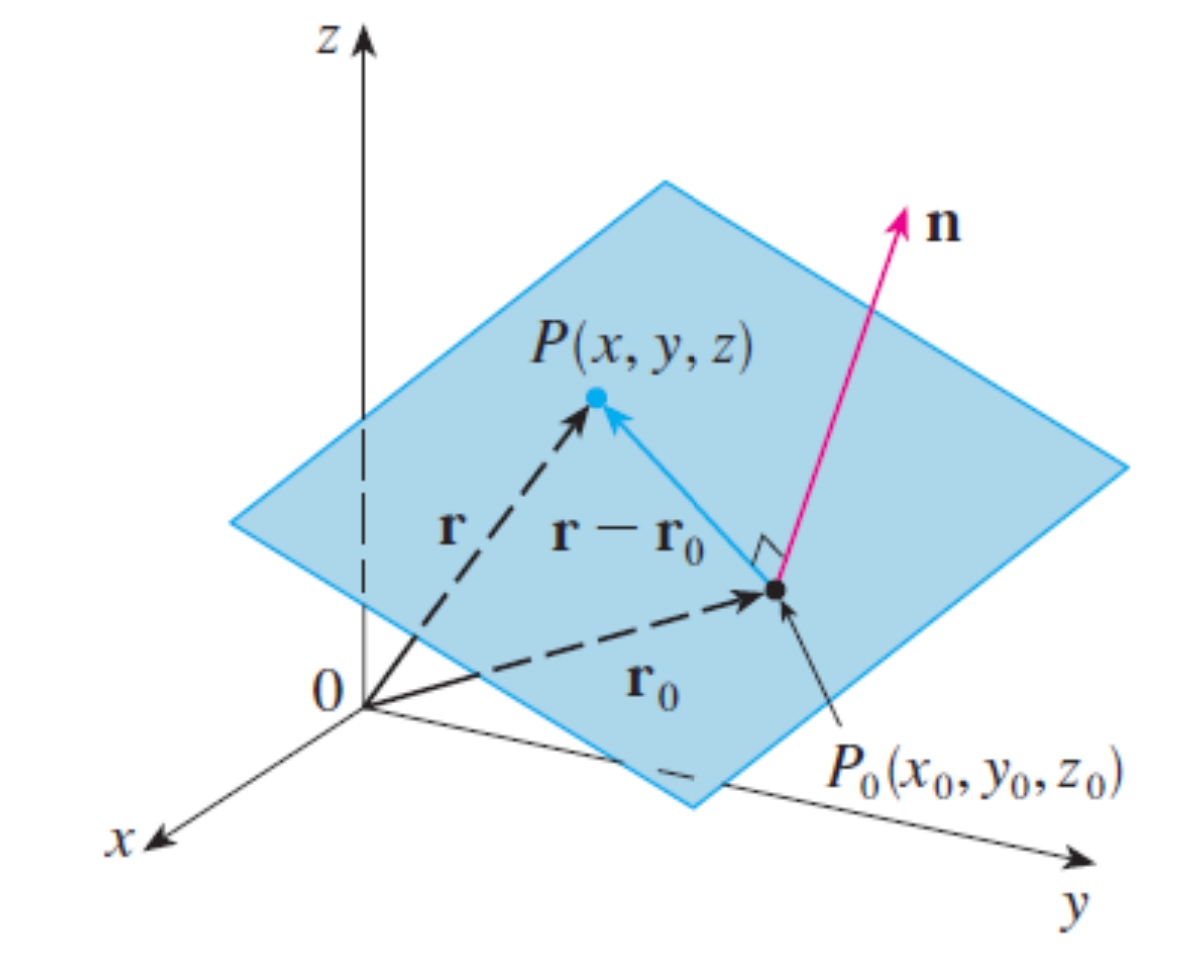
\includegraphics[width=7cm]{3d_plane.png}
\caption{Illustration of a plane}
\label{fig:plane}
\end{center}
\end{figure}


\subsection{Task 1.3}

Given a plane $s$ defined by equation 
$\mathbf{r} = 
\begin{bmatrix} 2 \\ 2 \\ 2 \end{bmatrix} + 
t \begin{bmatrix} -2 \\ 3 \\ 3 \end{bmatrix} + 
u \begin{bmatrix} 1 \\ 1 \\ -5 \end{bmatrix}$, find equation of a line $l$, perpendicular to $s$ and passing though the origin. Find a projection of the point $\mathbf{g} = \begin{bmatrix} -10 \\ -3 \\ 5 \end{bmatrix}$ on $l$.


\subsection{Task 1.4}

Given a plane $s$ defined by equation 
$\mathbf{r} = 
\begin{bmatrix} -5 \\ 11 \\ 0.5 \end{bmatrix} + 
t \begin{bmatrix} 1 \\ 0 \\ 0 \end{bmatrix} + 
u \begin{bmatrix} 4 \\ 2 \\ -1 \end{bmatrix}$, and a point $\mathbf{g} = \begin{bmatrix} -10 \\ -3 \\ 5 \end{bmatrix}$, find a point $\mathbf{g}^*$ symmetrical to $\mathbf{g}$ relative to the plane $s$.



\section{Task 2}

Given a system of equations

\begin{equation}
    \begin{cases}
    3x+y+z=0 \\
    6x+2y+2z=0 \\
    -9x-3y-3z=0
    \end{cases}
\end{equation}

we define its space of solutions as $V$.


\subsection{Task 2.1}

Find a basis in $V$. Visualize $V$ as a plane.

\subsection{Task 2.2}

Given an arbitrary vector $\mathbf{g}$, write a procedure of how to find its orthogonal projection onto $V$, and onto the orthogonal compliment of $V$. Prove that the procedure you propose is correct. Show the projection results for $\mathbf{g} = \begin{bmatrix} -1 \\ -1 \\ 3 \end{bmatrix}$. Visualize the projection.

\subsection{Task 2.3}

Let $\mathbf{g}^{||}$ be the orthogonal projection of the vector $\mathbf{g}$ onto $V$, and $\mathbf{g}^\perp$ be the orthogonal projection of the vector $\mathbf{g}$ onto the orthogonal compliment of $V$. With that information, how can we recover $\mathbf{g}$? Prove that your procedure is correct.

\section{Task 3}

You are given the following optimization problem:

\begin{equation}\label{eq:qp}
\begin{aligned}
 \min_{x_1,x_2} \quad &   \frac{1}{2} x_1^2 + 4x_2^2 -32x_2 + 60 \\
\textrm{s.t.} \quad  & x_1 + x_2 \leq 6 \\
  \quad &  x_1 + 2x_2 \leq 8\\
  \quad &  x_1 \geq 0 , x_2 \geq 0,  x_2 \leq 9,
\end{aligned}
\end{equation}

\subsection{Task 3.1}

Rearrange the problem (\ref{eq:qp}) in the following form 

\begin{equation}\label{eq:qp2}
\begin{aligned}
 \min_{\mathbf{x}} \quad &   f(\mathbf{x}) = \frac{1}{2}\mathbf{x}^T H  \mathbf{x} + c \mathbf{x} + c_0 \\
\textrm{s.t.} \quad  & A \mathbf{x} \leq b \\
\end{aligned}
\end{equation}

\subsection{Task 3.2}

Use CVXPY to solve both \eqref{eq:qp} and \eqref{eq:qp2}. 

\subsection{Task 3.3}

Visualize the domain of the function, its cost function and its solution.

\section{Submition}

Please upload the single zip file which includes your source code and the report. 

\section{Deadline}
The deadline: April 18, 23:59:59 GMT+3.

\end{document}